\documentclass[onecolumn, draftclsnofoot,10pt, compsoc]{IEEEtran}
\usepackage{graphicx}
\usepackage{url}
\usepackage{setspace}

\usepackage{geometry}
\geometry{textheight=9.5in, textwidth=7in}

\usepackage{listings}
\usepackage{color}

\definecolor{dkgreen}{rgb}{0,0.6,0}
\definecolor{gray}{rgb}{0.5,0.5,0.5}
\definecolor{mauve}{rgb}{0.58,0,0.82}

\lstdefinestyle{php}
{
   frame=tb,
   language=PHP,
   aboveskip=3mm,
   belowskip=3mm,
   showstringspaces=false,
   columns=flexible,
   basicstyle={\small\ttfamily},
   numbers=none,
   numberstyle=\tiny\color{gray},
   keywordstyle=\color{blue},
   commentstyle=\color{dkgreen},
   stringstyle=\color{mauve},
   breaklines=true,
   breakatwhitespace=true,
   tabsize=3
}

\lstdefinestyle{java}
{
   frame=tb,
   language=C++,
   aboveskip=3mm,
   belowskip=3mm,
   showstringspaces=false,
   columns=flexible,
   basicstyle={\small\ttfamily},
   numbers=none,
   numberstyle=\tiny\color{gray},
   keywordstyle=\color{blue},
   commentstyle=\color{dkgreen},
   stringstyle=\color{mauve},
   breaklines=true,
   breakatwhitespace=true,
   tabsize=3
}

% 1. Fill in these details
\def \CapstoneTeamName{		The Cleverly Named Team}
\def \CapstoneTeamNumber{		14}
\def \GroupMemberOne{			Omeed Habibelahian}
\def \GroupMemberTwo{			Bradley Imai}
\def \GroupMemberThree{			Dylan Tomlinson}
\def \CapstoneProjectName{		"I Heart Corvallis" Mobile Application}
\def \CapstoneSponsorCompany{	Corvallis Community Relations Office}
\def \CapstoneSponsorPerson{		Lyndi-Rae Petty}

% 2. Uncomment the appropriate line below so that the document type works
\def \DocType{		%Problem Statement
				%Requirements Document
				%Technology Review
				%Design Document
				Progress Report
				}

\newcommand{\NameSigPair}[1]{\par
\makebox[2.75in][r]{#1} \hfil 	\makebox[3.25in]{\makebox[2.25in]{\hrulefill} \hfill		\makebox[.75in]{\hrulefill}}
\par\vspace{-12pt} \textit{\tiny\noindent
\makebox[2.75in]{} \hfil		\makebox[3.25in]{\makebox[2.25in][r]{Signature} \hfill	\makebox[.75in][r]{Date}}}}
% 3. If the document is not to be signed, uncomment the RENEWcommand below
\renewcommand{\NameSigPair}[1]{#1}

%%%%%%%%%%%%%%%%%%%%%%%%%%%%%%%%%%%%%%%
\begin{document}
\begin{titlepage}
    \pagenumbering{gobble}
    \begin{singlespace}
    	\includegraphics[height=4cm]{coe_v_spot1}
        \hfill
        % 4. If you have a logo, use this includegraphics command to put it on the coversheet.
        %\includegraphics[height=4cm]{CompanyLogo}
        \par\vspace{.2in}
        \centering
        \scshape{
            \huge CS Capstone \DocType \par
            {\large\today}\par
            \vspace{.5in}
            \textbf{\Huge\CapstoneProjectName}\par
            \vfill
            {\large Prepared for}\par
            \Huge \CapstoneSponsorCompany\par
            \vspace{5pt}
            {\Large\NameSigPair{\CapstoneSponsorPerson}\par}
            {\large Prepared by }\par
            Group\CapstoneTeamNumber\par
            % 5. comment out the line below this one if you do not wish to name your team
            %\CapstoneTeamName\par
            \vspace{5pt}
            {\Large
                \NameSigPair{\GroupMemberOne}\par
                \NameSigPair{\GroupMemberTwo}\par
                \NameSigPair{\GroupMemberThree}\par
            }
            \vspace{20pt}
        }
        \begin{abstract}
        % 6. Fill in your abstract
        		This document takes a look back at the work we have done on the I Heart Corvallis mobile application this past term. It recaps the purposes and goals of the application, explains where we are currently on the project, and describes problems we have faced so far, how they impeded our progress on the project, and how we solved those problems. It also highlights several useful pieces of code we encountered throughout the research process and provides a retrospective of the past 6 weeks, looking back at the positives that happened each week, any changes we need to implement in our project, and what we will do to successfully make those changes.
        \end{abstract}
    \end{singlespace}
\end{titlepage}
\newpage
\pagenumbering{arabic}
\tableofcontents
% 7. uncomment this (if applicable). Consider adding a page break.
%\listoffigures
%\listoftables
\clearpage

% 8. now you write!
\section{Project Overview}
	The I Heart Corvallis project is a mobile application we are creating for the Corvallis Community Relations office (also known as the CCR office) and is part of a larger Initiative ran by the office to help students become more involved in the Corvallis community. The application focuses on increasing student awareness of events and service opportunities happening around Corvallis, as well as creating an incentive for students to attend these events. \\ \\
	On top of listing events and service opportunities available to users, the application provides users with a passport that shows them which events they’ve completed. Users receive stamps upon completing events, and when a user accumulates a certain number of stamps, they can turn in their stamps for rewards. \\ \\
	The application also presents users with community resources available to them, a map of notable community establishments and locations, and more information about the I Heart Corvallis initiative.

\section{Current Status}
	Currently, we have finished majority of the application interface which will be discussed below in each of our individual progress reports. The main features left to implement are the geolocation, security, authorization of event attendance and small features to the administration website.

\section{Problems We've Encountered}
	One of the first problems we encountered when implementing our application was where to host our database. We had figured that we would be able to host our database on our ONID accounts however, our accounts would only be able to last for a year or so after we graduate which would be a problem for our clients. Another issue that has been coming up is our client bringing up small changes to the application. Which is not too big of problem but all of these small changes continue to add up in the end. And lastly, we would like to be able to access student onid logins for our login page so that students will not have create new accounts for our app. Unfortunately we are still unsure if we have permission from the university to utilize the CAS ONID login system.

\section{Solutions to Problems}
	In order to solve these problems we’ve either done research, met with people who have done the research, or have made plans to meet with people. The first person we met up with was Derek Whiteside, the director of web and mobile services for OSU. As a group we discussed hosting our database on one of their servers. Unfortunately they were not able to help us as they dont really allow random projects to hang out on their servers, but we did receive a lot of good feedback to our application, including who to talk to about the CASS (or ONID) login and who to contact regarding using oregon state branding. After that discussion with Derek we decided to take his advice and have our clients go to a third party to host the database. As of now we are still hosting our data on our ONID accounts. In the near future we plan on meeting up with Kegan Sims to discuss OSU branding.  In regards to our clients adding small changes, we have set up weekly meetings in order to discuss changes we’ve implemented and future changes to ensure that we are creating this application in a way that our clients approve of.

\newpage
\section{Bradley}
	\subsection{Map Integration}
		Throughout our discussions with our client during fall term, Lyndi presented us with a map that displayed useful resources and notable locations. She had asked us to replicate these maps into the application. To my knowledge at the time, I had figured that I would be able to take the map from the website and display it onto the application. However, I ran into some trouble with displaying the map and had to rethink my implementation of it. In the end, I created two separate maps using the Google Maps API. The first map I created was the resource map. In order to display the notable landmarks on to this map, I first hard-coded each of the markers by its latitude and longitude in the Java file. Later on, I was able to figure out that you can use AsyncTask to retrieve the data from the database instead of hardcoding the latitude and longitude within the Java file. The second map I created was for the events page. This map displays the current list of events that are happening on the events page list. \\ \\

		\includegraphics[height=8cm]{resourcemap}

	\subsection{Splash Screen}
		One of the simplest and neatest features that I implemented into this application was the splash screen. Even though it is a simple feature, it still took me a little time to figure out and implement it into the application. The splash screen occurs when the user first opens the app. A quick animation is created which gives the application a more fluid transition to the login page. If the user does not close the application, the animation will not appear, however, if they do close the application and reopen it, the animation will be displayed. When I showcased the feature to our client she was very impressed and loved the animation.

		% ADD SPLASH SCREEN SCREENSHOT

	\subsection{Administrative Website Functionality}
		Most recently our client suggested that she and the Corvallis Community Relations office need to be able to manage in-app content through an administrative website. I took upon this task and created an admin website were our clients would be able to access this data. I first started off with the home page and the main page. On this page our client will have the option to add an event, manage events, manage primary resources, manage resource map, add a prize or manage prizes. As of now, our client is only able to access the “Add an Event” and “Manage Events” pages. I am currently in the process of implementing the other pages. Once I created the layout of the home page I began the implementation of the add events section. This section is where the client is able to add in new events to the database which are then displayed in the events section of the application. In order for our client to add an event successfully I had to connect the database to our website. With the help of Omeed, I was able to successfully connect the database to the website via PHP. The fields that are listed are event name, name of a location, full address, date, time (am, pm), description of an event, image, links and a pin. Our client will be required to fill in all of the red asterisk fields in order to add an event to the database. Once the client submits the event, they will receive a message saying the event has been successfully added. I plan on creating a pop-up message saying, “Event has been successfully added!” rather than redirecting them to another page. \\ \\

		\includegraphics[height=9cm]{websiteaddevent}

		Moving onto the Manage Events section of the website, our clients will be able to edit or delete any existing events. It currently displays all of the events in the database and provides action buttons (editing and deleting) by each event. If the client wishes to edit an event they will click the edit button which will direct them to another page. The secondary page will list the name, location, date and time of the event in which they can re-edit. Once the client resubmits the event, the event will then be updated in our database and a pop-up message saying "Event is successfully added!" will appear. If the client wishes to remove an event, they can simply click the remove button and a confirmation message will pop up stating, “Are you sure you want to delete this event?”, if so the client can click ok and the event will be removed from the web page and database. \\ \\

		\includegraphics[height=5cm]{websitemanageevents}

		I will continue to work on the other functionalities of the website such as adding a marker to the resource map page, allow the client to edit the content on the resource page, and create a login for our client. In order to add a new marker/pin to the resource map, I plan on promoting our client with the specific fields, name and location/address of the place. I will then retrieve that information and implement a function that takes in the address and stores the address as a longitude and latitude into the database in which it will then be displayed on the application. Very similar to the manage events page, I will allow our client to edit the information on the resource page such as editing links, photos, and texts. Lastly, I will create a login page that only our client and the CCR office would be granted access to. \\ \\

		\includegraphics[height=6cm]{websitehomepage}

	\subsection{Geolocation}
		In the upcoming weeks, I also plan on implementing the feature of retrieving a current user’s location as well as creating a geofence. By obtaining a user’s current location, users will be able to view various events that are happening around them. This feature will also serve as a secondary checker along with the PIN to verify that the user is at that event. For example, if a user hikes Bald Hill, our client will work with the city of Corvallis to have a sign set up at the top of the hill that states “Check in here on the I Heart Corvallis app!” We will then check the user’s location, and prompt them with a little button that says, “check in” and they will then be given the stamp for completing the Bald Hill Hike.

\newpage
\section{Omeed}
	\subsection{Database Usage}
		In order to display content in a consistent manner across all devices and to allow for changes to in-app content to be mirrored on all devices, we rely on database tables for storing our data remotely. User information is stored in a table called “ihc\_users,” as shown below. Event information is stored in “ihc\_events,” records for completed events are stored in “ihc\_completed\_events,” prize information is stored in “ihc\_prizes,” and resource map information is stored in “ihc\_resources.” We will be creating another table to hold the content that gets displayed on the main resource page as well. For now, these tables are stored in my ONID database, but they will soon be moved to a third-party database so that they remain accessible after we graduate and leave OSU. \\ \\

		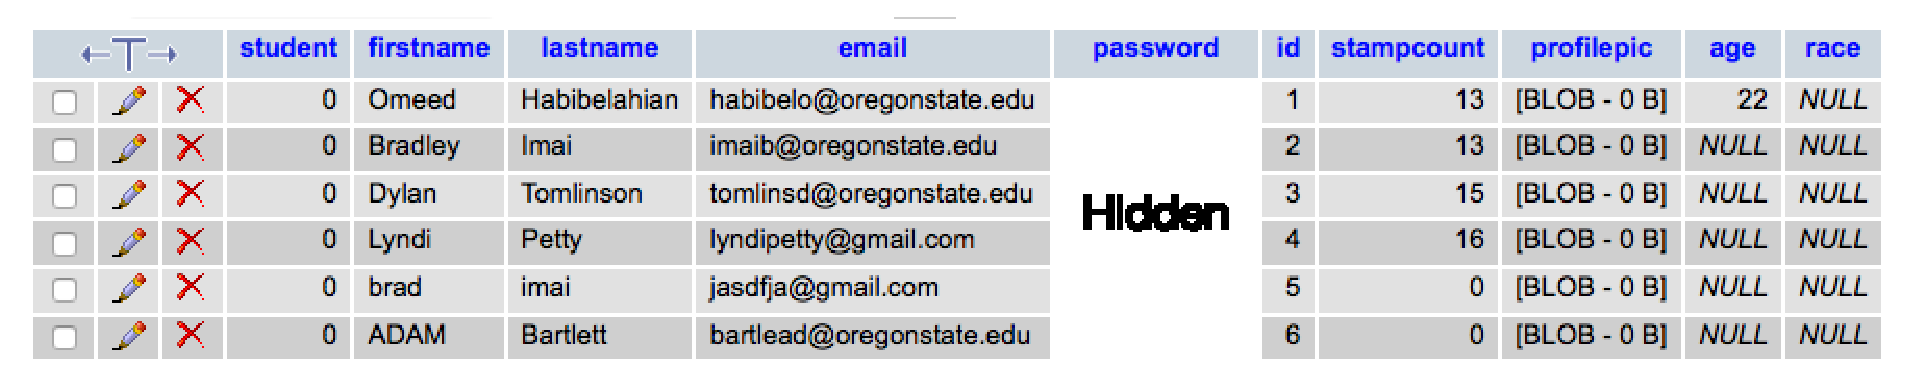
\includegraphics[height=3cm]{ihcusersdb}

		Since the application cannot directly access the database, we have many PHP scripts stored on the ENGR server that act as a middle man between the app and the database. The app sends values up to the PHP scripts using an HTTP POST request, and the PHP script uses these values to search for specific information in the appropriate database table. The script either echoes the desired values or messages back down to the application or echoes an error message back down, and the app reads this message and acts accordingly. \\ \\
		For example, when a user logs in, if their email and password combination is in the users table, the script echoes down the user’s information (excluding their password) down to the app, which creates a new object of the User class (a class we have created to hold user info) and stores this information in that object, along with a “LOGINSUCCESS” message, which the app looks for to see if the login attempt was successful. If the user is not found in the database, or if another searching error occurs, the script echoes down the appropriate error message, which the app handles appropriately. The bulk of this PHP script is shown below.
		\newpage

		\begin{lstlisting}[style=php]
$email = $password = $row = "";

if ($_SERVER["REQUEST_METHOD"] == "POST") {
	$email = $_POST['email'];
	$password = $_POST['password'];

	$result = $mysqli->query("SELECT email, password FROM ihc_users");
	if ($result->num_rows > 0) {
		while ($user = $result->fetch_assoc()) {
			if ($user["email"] == $email && $user["password"] == $password) {
				$isAuth = True;
				break;
			}
		}
	}
	if ($isAuth == True) {
		$result = $mysqli->query("SELECT firstname, lastname, email, id, stampcount FROM ihc_users WHERE email='$email' AND password='$password'");

		if ($result->num_rows == 1) {
			while ($row = $result->fetch_assoc()) {
				$data = json_encode($row);
				echo "LOGINSUCCESS\\";
				echo $data;
			}
		}
		else if ($result->num_rows == 0) {
			echo "NOACCOUNTERROR"; # account does not exist
		}
		else if ($result->num_rows > 1) {
			echo "DUPACCOUNTERROR";  # more than one account with this email/password
		}
		else {
			echo "SEARCHERROR"; # error looking for account
		}
	}
	else {
		echo "AUTHERROR"; # unable to authenticate email/password
	}
}
		\end{lstlisting}
		\newpage

		On top of the app’s usage of values from the database, the administrative website also heavily relies on the database. Our client needs to be able to add, modify, and delete events, resource information, resource map pins, and prizes. Therefore, connection to the database is crucial to enable our client to manipulate data, as without this integration they would have to log into the database itself and modify information on that interface, which would likely be significantly less intuitive than manipulating this content on our administrative website.

	\subsection{User Interface Setup}
		When the user first opens the app, they are shown a introductory splash page that shows the app logo. After a few seconds, if they are not logged in, the app automatically takes the user to the page that lets them choose to log in or sign up. If they are logged in, the app instead automatically takes them directly to their dashboard. Most of the pages behind the login wall are aesthetically set up in the same way. The page has a black toolbar containing the title of that page, the navigation button (or back arrow in some cases), and any other action button relevant to that page. The content is generally shown with a white background and black text, and most of the content is displayed in a list format, which we implement using Android’s RecyclerView class. We also utilize the CardView to display events in card form. Events are displayed in a list format by default, but the user can choose to see events in card form. \\ \\
		We also implement Google Maps on the Events page and the Resource page. On the main Events page, the user can press the map icon on the right corner of the app’s toolbar to open a map centered on Corvallis that shows the locations of all of the events listed in the app, with each event represented by a map marker. If the user is on the detailed page for a particular event, the map icon instead opens a map centered on that event’s location that solely shows a marker for that event.

	\subsection{Administrative Website Structure}
		I have designed the administrative website to be visually and structurally simple to use, since the CCR office does not have a lot of technical prowess. For a clean, easy-to-use and easy-to-implement visual interface, I utilized Semantic UI, which provides a vast library of interface elements like tables, buttons, and icons. For pages that allow for the addition of content, the site provides text boxes for all major pieces of information. For example, on the “Add an Event” page, the page provides text boxes for event elements such as name, location, address, date and time, description, image, and up to three important links. It also lets our client randomly generate a 4-digit PIN that will be used to verify that a user went to that event. \\ \\
		For pages that allow for the modification and deletion of content, our client can see every event, resource, resource map element, or prize (depending on the page) stored in the database, and they have the option to edit or delete the element. If they choose to edit the element, they are taken to page that is visually identical to the addition page, except the input boxes are pre-populated with the current values for that element. Upon clicking Submit, that element will be updated in the database. If they instead choose to delete the element, they will get a confirmation message, and if they click “OK,” that element will be removed from the database.

	\subsection{Login/Signup}
		Upon opening the app for the first time or logging out of their account, the user will be given the option to log into their account or sign up for a new account. If they choose to log in, they will be given the option to go to the student login page or the non-student login page. If the user chooses the student login, they will be directed to page where they can enter their ONID username and password to log into their account. Otherwise, they will be taken to a page where they can enter their non-student email and password. If the user instead chooses to sign up, they will be taken to a page where they can enter their first and last name, email, and password. In the future we may also add some simple introductory questions for the user such as age, race, etc. These questions would be stored in the database for analytical use by our client. Upon filling in all the fields of the form, the app will send these values to the appropriate PHP script, which will confirm or deny that this account already exists. If the account does not already exist, the user’s account will be initialized and they will be taken to their dashboard. OSU students will have the option to bypass the majority of this signup form and use their ONID username and password to make an account. \\ \\

		\includegraphics[height=8cm]{nonstudentlogin}
		\includegraphics[height=8cm]{signup}

\newpage
\section{Dylan}
	\subsection{Action Toolbar, Navigation Menu, and Initial Page Designs}
		To begin the project, we met up several times during the winter break to set up the initial parts of the project. There was a lot of overhead that we had to figure out before we could start knocking off requirements. During this time I worked on a few small changes for the app. I added in a few required java classes such as the logout and login classes with no implementation. I also put in the initial onCreate functions and the required inputs for the rest of the pages in these initial steps. After this I worked on creating the navigation menu that slides out from the side as seen below. \\ \\

		\includegraphics[height=8cm]{navigationmenu}

		It first required to change the default toolbar to an action toolbar, which would allow us put any custom buttons on it. After making those changes I added more of the base code necessary for the navigation menu. I added the changes to make the menu scroll out when you click its button and I added a few of the pages on the navigation menu. Omeed completed the rest of the implementation by adding in the actual links in the menu, icons to the links, and adding a delay to the menu slide so that it appears fluid. The next thing I worked on began after the start of the term. I put in formatting and content on secondary pages so that we could get a more concrete prototype to show our client. This simply entailed adding in relative layouts and text views with a few buttons and hard coding some basic text. I also added in a table view for the leaderboard and passport pages. This was a useful step in helping us decide what our interface was going to look like for each of these pages.

	\subsection{RecyclerView}
		After that I implemented a recycler layout for the leaderboards page. The recycler layout helps reduce the amount of processing power needed for pages that are populated with long lists of items. This required creating an adapter class to systematically generate new views to host the content. Our leaderboard page pulls in all of the user accounts from the database and displays their names along with their stamp counts, so it is one of the pages that will benefit from this change. \\ \\

		\includegraphics[height=8cm]{eventlistview}
		\includegraphics[height=8cm]{eventcardview}
		\includegraphics[height=8cm]{passport}
		\includegraphics[height=8cm]{leaderboard}

	\subsection{Updating the Design Document}
		The next thing I worked on was updating the design document with Bradley. We made some big changes to the design of our project back during the winter break. We were originally going to implement the UI with the Semantic UI library, but we eventually found out that this would require us to basically convert our program from a website to an application. This added a lot of extra processing for our app which would make it a lot slower than simply using the android SDK. We ended up doing just that, and needed to include those changes in our design document.

	\subsection{Session Management}
		The next thing I worked on was the logout capability and session management. At the time we could log in to our application but we could never log out. To do this the program needed to somehow know that the user was logged in, in order to log them out. This required what is called a session. When a user successfully logs into their account, a session is automatically created for them.
		\newpage

		\begin{lstlisting}[style=java]
private void onBackgroundTaskDataObtained(String result) {
	if (result.contains("LOGINSUCCESS")) {
      try {
      	StringTokenizer st = new StringTokenizer(result);
         String returnMsg = st.nextToken("\\");

         String userInfo = st.nextToken("\\");
         JSONObject userJSON = new JSONObject(userInfo);
         String first = userJSON.getString("firstname");
         String last = userJSON.getString("lastname");
         String name = first + " " + last;
         String email = userJSON.getString("email");
         session.createLoginSession( name , email);
         Intent intent = new Intent(NonStudentLoginActivity.this, DashboardActivity.class);
         startActivity(intent);
      } catch (Exception e) {
         Toast.makeText(this, "Exception: " + e.getMessage(), Toast.LENGTH_LONG).show();
      }
   }
   else {
		// Check for error message (this section has been omitted in this paper for compactness and to highlight the important code, which is in the "if" block)
	}
}
		\end{lstlisting}

		The app does this by parsing through the string that is returned from the php script and tokenizes it. It then splits each token into string variables which are then passed into the creatLoginSession function. As shown here the strings that are passed are the user’s name and email. The user’s email and name are then stored in the session. The app loads this session on every other page of the app in order to use the information from it. Currently the only uses for the session are displaying the user’s name and email in the navigation menu,  deleting itself when a user logs out, and redirecting a user to the dashboard if they launch the app and were already logged in.
		\newpage

		\begin{lstlisting}[style=java]
public void logoutUser(){

	//clearing all data from shared preferences
	editor.clear();
	editor.commit();

	//after logout redirect user to main activity
	Intent i = new Intent(_context, MainActivity.class);

	//closing all the activities
	i.addFlags(Intent.FLAG_ACTIVITY_CLEAR_TOP);

	//add new flag to start new activity
	i.setFlags(Intent.FLAG_ACTIVITY_NEW_TASK);

	//starting login activity
	_context.startActivity(i);
}
		\end{lstlisting}

		This is the code that logs the user out. It is called when the user clicks the logout button on the settings page. It simply deletes the stored information it has gathered of the user, and sends the user to the welcome screen mainActivity. I also added functionality that allows each page to check if the user is logged in. If they are not then the application redirects them to the main activity page, where users can log in or sign up. I have not included it on any of the pages yet so that we do not have to log in every time to test our program, but it has been tested and it functions correctly.

	\subsection{Security}
		What I will be be working on next is implementing various security features for our application. I am going to begin with utilizing the Password-Based Key Derivation Function 2 hash, or PBKDF2. Currently I have implemented parts of this functionality. The app as of now hashes a user’s password when they create an account. It then stores the hashed password into the database, instead of their clear text password as was done before. I currently am in the process of validating a stored hash from our database so that a user can be authenticated when they attempt to log-in. All that is needed to be done is to return a user’s stored password hash from the database in order to determine its salt. This is important because we need to hash the attempted login password with the same salt that was used to hash the user’s original password. We will then be able to check if the entered password is the same as the stored password of the user’s account.  My next main objective will be to work on sanitizing any user inputs to prevent SQL injections.

	\subsection{Interface Scaling}
		The last part of the project that I am specifically tasked with is ensuring that our application scales for different android devices. We want to make sure that anyone with an android phone that supports kitkat (android 4.4) can run our application. We also want to make sure that the application’s interface is still intuitive and fully functional. Lastly I will be working on general functionality of the application that will be written about in our final progress report for this term. There is still a decent portion of the project that needs to be completed, but these parts are rather small and will be divided among us as we get to them.



\end{document}
